\begin{tikzpicture}[align=center,
    arrow/.style={draw, thick, -{Latex[length=2mm]}},
    arrowr/.style={draw, thick, {Latex[length=2mm]}-}]
    \node[inner sep=0, rectangle] (user) {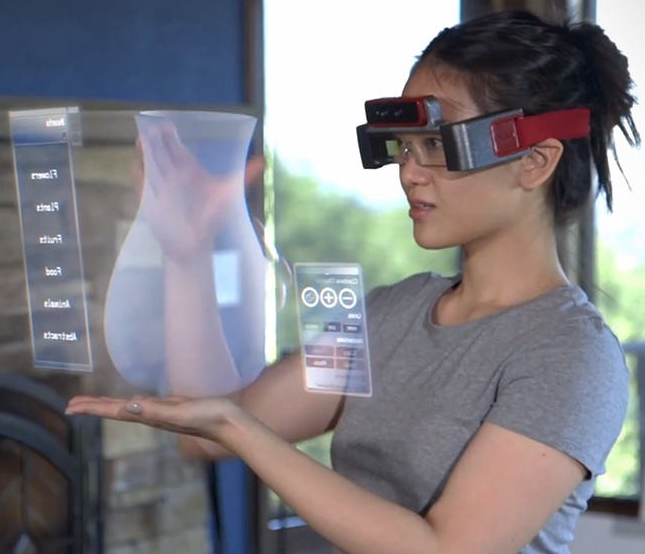
\includegraphics[width=.35\linewidth]{img/ar_glasses.png}};

    \matrix[inner sep=0mm, 
    left=2.5em of user, row sep=1em,
    nodes={rectangle, draw, text width=8em, rectangle, inner sep=2mm, thick, rounded corners=.7mm, fill=C2}] (lmtx) {%
        \node (performance) {Task performance};\\
        \node (errors) {\# of Errors};\\
        \node (time) {Task completion time};\\
    };

    \matrix[inner sep=0mm, 
    right=2.5em of user, row sep=1em,
    nodes={rectangle, draw, text width=8em, rectangle, inner sep=2mm, thick, rounded corners=.7mm, fill=C4}] (rmtx) {%
        \node (confusion) {Confusion};\\
        \node (annoyance) {Annoyance};\\
        \node (fatigue) {Fatigue};\\
    };

    % circles
    \node[circle, draw, thick, minimum height=4em, left=.5em of user.center] (task) {};
    \node[circle, draw=red, thick, minimum height=4em, left=1em of user.25] (head) {};
    \node[circle, fill=black, minimum height=.1mm, inner sep=1mm] at (task.west) {};
    \node[circle, fill=red, minimum height=.1mm, inner sep=1mm] at (head.east) {};

    \begin{scope}[every path/.style=arrowr]
        \path (performance.east) -- (task.west);
        \path (errors.east) -- (task.west);
        \path (time.east) -- (task.west);
    \end{scope}

    \begin{scope}[every path/.style=arrowr, draw=red]
        \path (confusion.west) -- (head.east);
        \path (annoyance.west) -- (head.east);
        \path (fatigue.west) -- (head.east);
    \end{scope}
\end{tikzpicture}